\subsection{Peer-to-Peer}

Als weitere Möglichkeit besteht eine Peer-to-Peer Architektur. Der Vorteil dieser ist, dass eine sehr gute Skalierbarkeit vorhanden ist. Zusätzlich bietet diese eine gute Robustheit. Da jeder Peer sowohl Geber als auch Nehmer ist, kann eine Replikation und somit auch eine Fehlertoleranz ermöglicht werden. Der größte Nachteil ist jedoch die Komplexität, sowie der Aufwand der Sicherheit.

Als Erweiterung zu normalen Peer-to-Peer Systemen gibt es DistributedHashTabels (DHTs). Diese verbessern die Skalierbarkeit und besitzen in der Suche keine \verb|false negatives|. Durch diese Besonderheiten, bietet sich eine DHT sehr gut an. Als einer der bekanntesten Algorithmen ist der CHORD bekannt, welcher die Hosts in einer Ringstruktur anordnet. Als Erweiterung zu diesem, werden sogenannte Fingertabellen hinzugefügt, welche Referenzen auf verschiedene Knoten haben. Ein Beispiel dieser Struktur ist in der folgenden Abbildung \ref{fig:chord} zu sehen.

\begin{figure}[h]
    \centering
    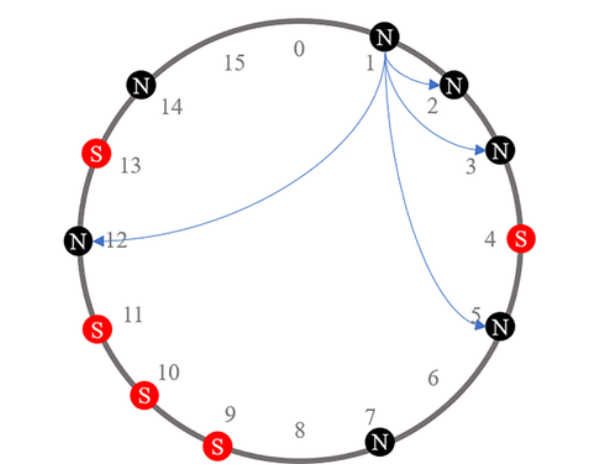
\includegraphics[width=0.5\textwidth]{chord.png}
    \caption{}{Beispielhafte Darstellung eines Chordrings mit vier Fingern\footnotemark}
    \label{fig:chord}
\end{figure}
\footnotetext{https://www.researchgate.net/figure/Chord-Ring-mit-Fingertabelle-eines-Elements\_fig1\_327512285}

Für die Implementierung ist man auf keine Programmiersprache oder ein bestimmtes Framework beschränkt. So kann über eine REST-Schnittstelle und einer Liste an Hosts, an welche sich gewendet werden kann, um beizutreten, die gesamte Struktur aufgebaut werden. Um ein Beispiel zu nennen, wäre Akka HTTP\footnote{https://doc.akka.io/docs/akka-http/current/index.html} eine gute Wahl für Java oder Scala.
